\section{Implementation, Room module}
The \textit{Room} functionalities are running on a ATM328P, the tasks of the module are implemented as pseudo-periodical tasks using the \textit{timer0} 
to check the activation time of each task, the tasks are reported in the following table.

\begin{center}
	\begin{tabular}{||c | c ||} 
		\hline
		Name 	& Frequency \\ 
		\hline
		\textbf{Main task}			&	0.5Hz \\ 
		\hline
		\textbf{ControlValve task}	&	0.25Hz \\ 
		\hline
	\end{tabular}
	\captionof{table}{Tasks running on the Room module \label{tab:RoomTasks}}
\end{center}

\begin{figure}[h]
	\centering
	\begin{subfigure}{0.4\textwidth} % width of left subfigure
		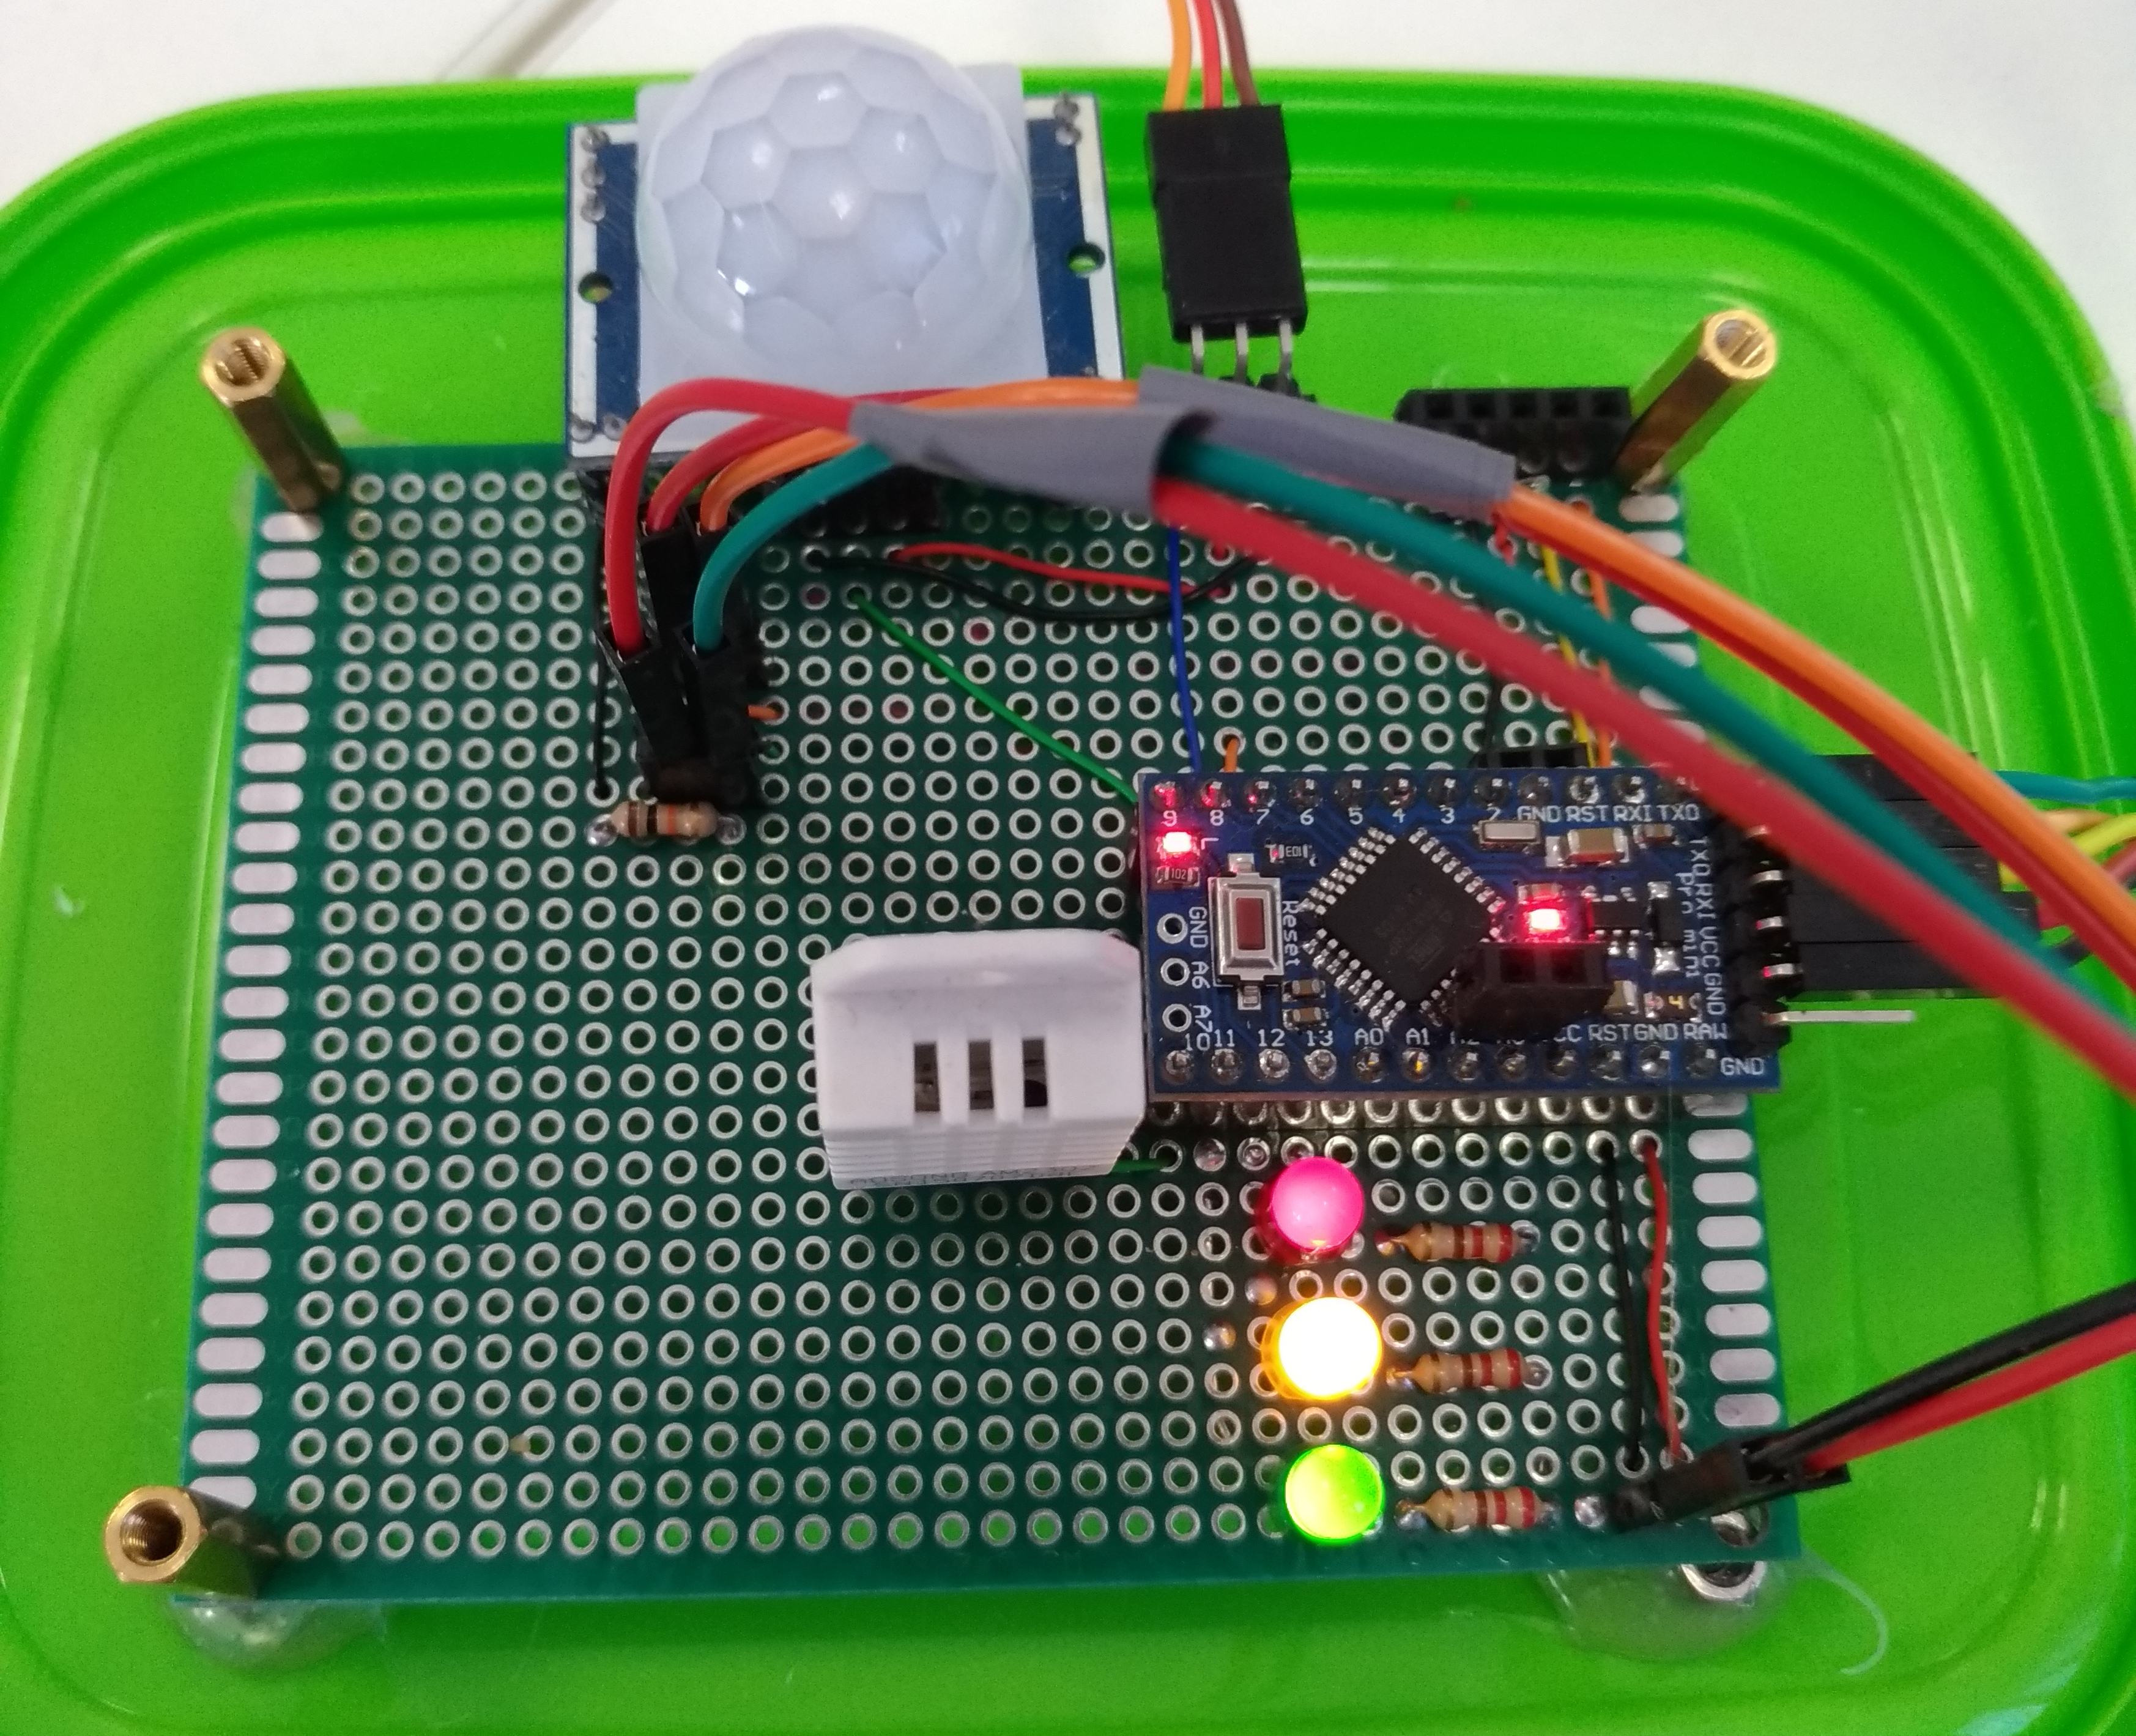
\includegraphics[width=4cm,keepaspectratio]{img/room_board}
		\caption{Room module}
		\label{fig:room_module}
		\end{subfigure}
	\vspace{1em} % here you can insert horizontal or vertical space
	\begin{subfigure}{0.4\textwidth} % width of right subfigure
		
\includegraphics[width=4cm,keepaspectratio]{img/valve}
		\caption{Valve}
		\label{fig:valve}
	\end{subfigure}
\end{figure}


The module is composed by:
\begin{itemize}
	\item Arduino pro mini, Atmega328P (8MHz, 3.3v logic)
	\item DHT22 Temperature and Humidity sensor
	\item PIR motion sensor
	\item Red led
	\item Green led
	\item Yellow led
	\item Servo Motor tower pro SG90
	\item 2 switch to check the open and closed position of the valve
\end{itemize}

\subsection{Components description}
\subsubsection{ServoMotor}
	\begin{figure}[h]
		\centering
		\begin{subfigure}{0.4\textwidth} % width of left subfigure
			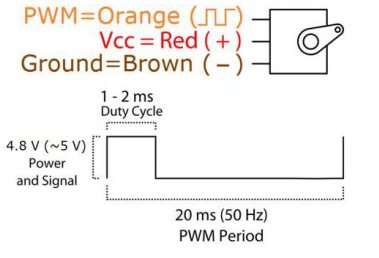
\includegraphics[width=4cm,keepaspectratio]{img/servo_signal}
			\end{subfigure}
		\vspace{1em} % here you can insert horizontal or vertical space
		\begin{subfigure}{0.4\textwidth} % width of right subfigure
			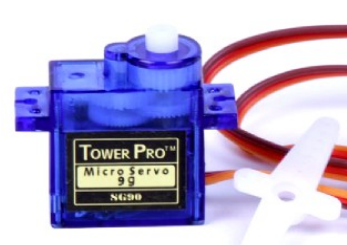
\includegraphics[width=4cm,keepaspectratio]{img/servomotor}
		\end{subfigure}
		\caption{Servo Motor}
		\label{fig:ServoMotor}
	\end{figure}

	The chosen ServoMotor is a Tower Pro SG90 reported in \ref{fig:ServoMotor},
	As reported in the \ref{fig:ServoMotor}, the signal used to move the servomotor in the correct position is a PWM and the duty-cycle describe the position that the motor has to maintain.
	The signal to control the motor position is managed by the Servo library using the \textbf{timer1} a 16-bit timer.
	The digital circuit inside the servomotor will adjust the position of the rotor using a potentiometer attached to that.
	In the following table are reported	the characteristics of the servomotor:
	\begin{center}
		\begin{tabular}{||l | l | l||} 
			\hline
			Voltage(V) & 4.8 - 6 \\ 
			\hline
			Torque(Kg-cm) & 2.5 \\
			\hline
			Speed(sec) & 0.1 \\
			\hline
			Weight(g) & 14.7 \\
			\hline
		\end{tabular}
		\captionof{table}{Servo motor characteristics \label{tab:ServoCharacteristics}}
	\end{center}

\subsubsection{Valve position switches}
\begin{figure}[h]
	\centering
	
\includegraphics[width=6cm,keepaspectratio]{img/valve}
	\caption{Discovery board wiring}
	\label{fig:valve}
\end{figure}
In order to check the position of the valve, two switches are fixed in the open and closed position, during the \textit{init\_valve} phase the possible positions are computed starting from the open and closed position.
Whenever the valve is in the open or closed position a check is done using the switches.

\subsubsection{Temperature-Humidity Sensor}
The sensor DHT22 have been used for the projet, in the following tables are reported the features of the sensors.
The sensor has a dedicated one-wire communication protocol implemented by the DHT adafruit library, a pull-up resistor is used in order to mantain the line clear when no one is transmitting.

\begin{center}
	\begin{tabular}{||l | l||} 
		\hline
		Voltage(V) & 3 - 5 \\ 
		\hline
		Current(mA) & 2.5 \\
		\hline
		Humidity(\%) & 0 - 100 \\
		\hline
		Humidity Accuracy(\%) & 2 - 5 \\
		\hline
		Temperature(C\degree) & -40 - 80 \\
		\hline
		Temperature Accuracy(C\degree) & +/- 0.5 \\
		\hline
		Sampling rate(Hz) & 0.5 \\
		\hline
	\end{tabular}
	\captionof{table}{DHT22 characteristics \label{tab:DHT22Characteristics}}
\end{center}


\subsection{Wiring}
	\begin{figure}[h]
		\centering
		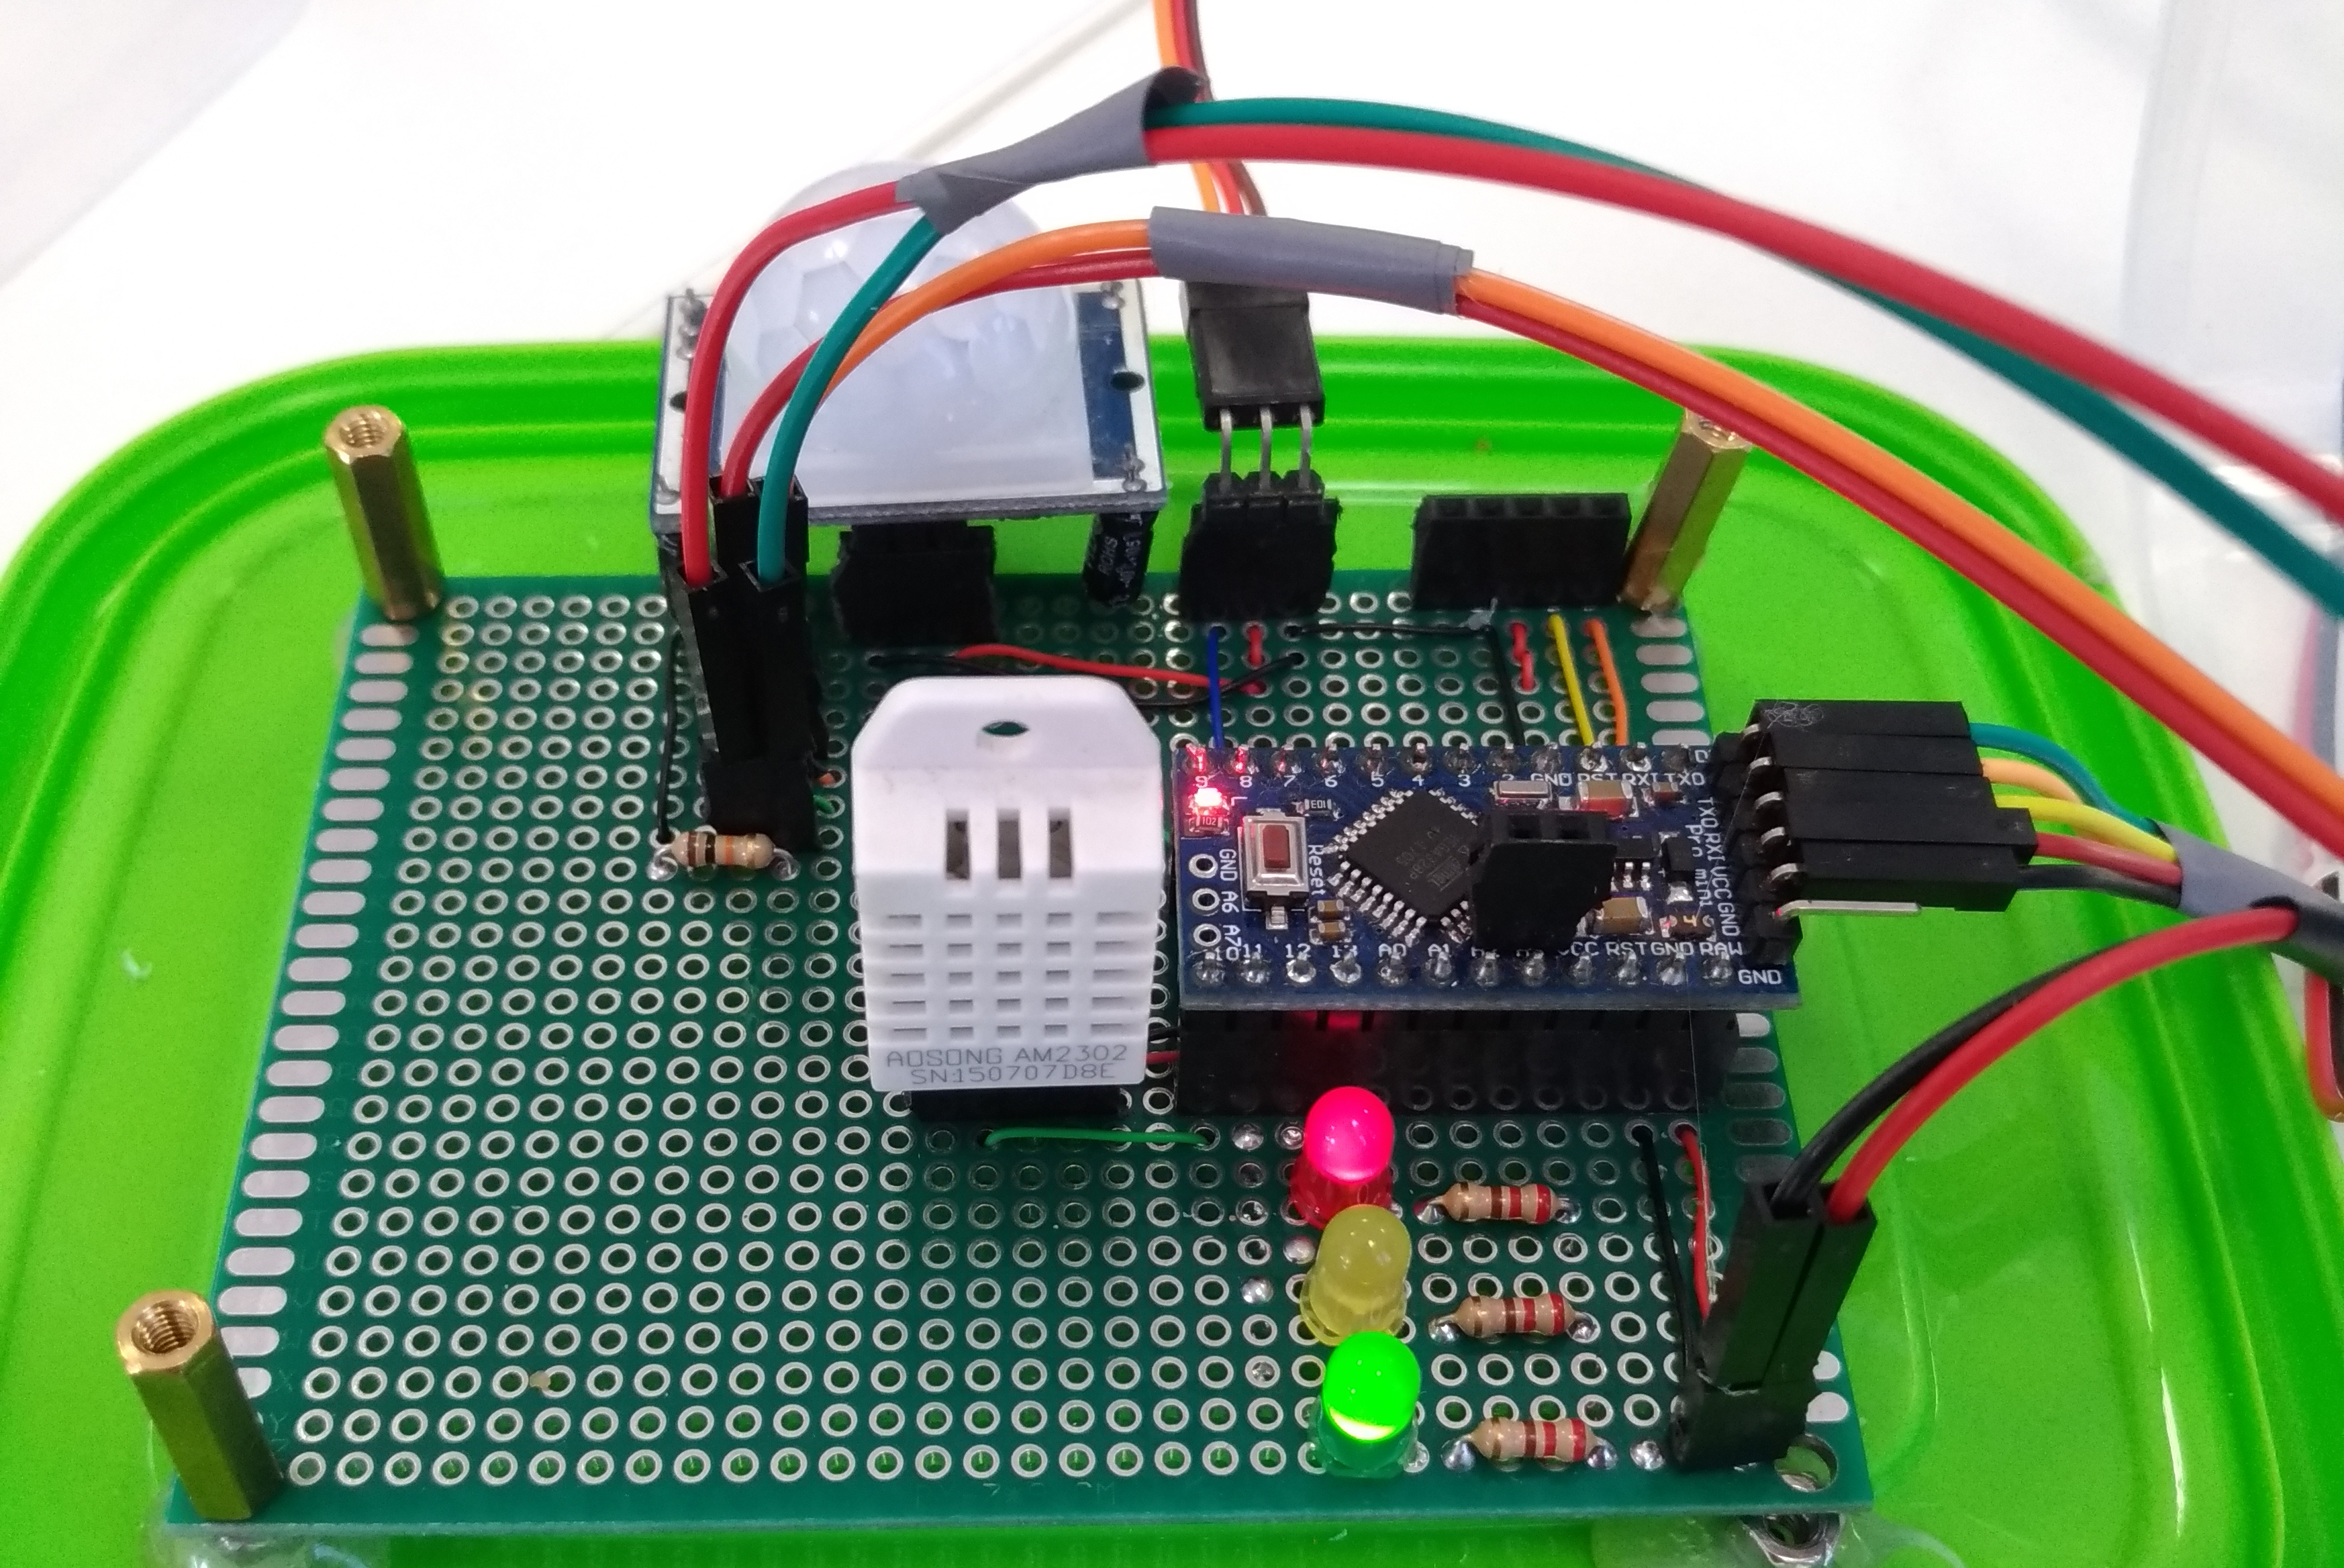
\includegraphics[width=6cm,keepaspectratio]{img/room_board_wiring}
		\caption{Room board wiring}
		\label{fig:room_wiring}
	\end{figure}
	The board is powered by 5V external power attached to the \textit{Raw pin}, this source is shared with the servomotor and the PIR sensor.
	In \ref{fig:room_wiring} is reported a picture of the implementation, in the following table the pins' configuration.
	\begin{center}
		\begin{tabular}{||l | l | l ||} 
			\hline
			Red led 			& 13 & D OUTPUT\\ 
			\hline
			Yellow led 			& 12 & D OUTPUT\\
			\hline
			Green data 			& 11 & D OUTPUT\\ 
			\hline
			DHT data 			& 10 & D INPUT\\ 
			\hline
			PIR data 			& 9 & D INPUT\\ 
			\hline
			ServoMotor PWM 		& 8 & D OUTPUT\\ 
			\hline
			Open Switch 		& 7 & D INPUT\\ 
			\hline
			Closed Switch 		& 6 & D INPUT\\ 
			\hline
			USART TX	 		& 0 & D OUTPUT\\ 
			\hline
			USART RX 			& 1 & D INPUT\\ 
			\hline
		\end{tabular}
		\captionof{table}{Atmega328P Wiring \label{tab:Atmega328Pwiring}}
	\end{center}
	